\documentclass{article}
\usepackage{graphicx}
\usepackage{mathtools}
\usepackage{xfrac}
\usepackage{amsmath, amssymb}
\usepackage{listings}
\usepackage{float}
\usepackage{wrapfig}
\usepackage{tikz}
\usepackage{fullpage}
\usepackage{hyperref}
\usepackage{mathalpha}
\usepackage{tikz}
\usepackage{cite}
\usepackage{amsthm}
\usepackage{natbib}

\setcounter{section}{-1}

\newtheorem{theorem}{Proposition}[section]
\newtheorem{corollary}{Corollary}[theorem]
\newtheorem{lemma}[theorem]{Lemma}

\theoremstyle{definition}
\newtheorem{definition}{Definition}[section]

\theoremstyle{remark}
\newtheorem*{remark}{Remark}
\newtheorem*{example}{Example}
\newtheorem*{notation}{Notation}

\title{Fractals}
\author{David Lawton\\
        Lab Partner: Sami Lopez-Steffenson\\
        22337087}
\date{14th Oct. 2024.}

\begin{document}

\maketitle

\tableofcontents
\addcontentsline{toc}{section}{\numberline{}Abstract}
\begin{abstract}
        
\end{abstract}

\section{Keywords \& Preliminaries}\label{sec:keywords}
\begin{definition}
        An \textbf{`ideal' fractal} is a scale independent geometric object. Scale independent meaning that the scale on which the object is viewed does not affect the appearance.(\cite{LabHandbook})
\end{definition}
\begin{definition}
        A \textbf{`real' fractal} is a physical object which resembles a fractal one over certain scales. However, the object size sets an upper limit on the scale at which the fractal properties are observed, and of course, the resolution sets, a less defined, lower bound.(\cite{LabHandbook})
\end{definition}
\begin{definition}
        The \textbf{`fractal dimension'} of an object is a measure of it's commplexity, which is formally defined as
\begin{equation}
        \label{eq:fractal_dimension}
        D = \lim_{\varepsilon \to 0} \frac{\ln(N(\varepsilon))}{\ln(1/\varepsilon)}
\end{equation}
        where $N(r)$ is the number of units describing the object at scale $r/\varepsilon$.
\end{definition}
\section{Background \& Theory}\label{sec:background}
This labs concerns the analysis of fractal growth under varying conditions. The fractals in this experiment were grown as described in \ref{sec:methodology}, and then analysed using the box counting and mass-radius methods.\\
\indent The \textbf{box counting method} is a standard way of estimating fractal dimension. It involves covering the fractal with a mesh of mesh size $s = w/\varepsilon$, where $w$ is the width of the fractal and $\varepsilon$ is a scaling factor. The number of boxes $N(s)$ which contain part of the fractal is then counted. This is done for many values of $s$, until the boxes of a size such that they cannot be reduced further (pixel size) are reached. The fractal dimension is estimated by fitting a line to the graph of $\ln(N(s))$ against $\ln(s)$. The line is of the form
\begin{equation}
        \ln(N(\varepsilon)) = m\ln(s) + c
\end{equation}
We recall Eq. \ref{eq:fractal_dimension} and solve for $D=-m$ to find the fractal dimension.\\
\indent The \textbf{mass-radius method} is another method of estimating the fractal dimension of an object. A centre of the fractal is identified, and then a series of squares (for raster data) of width $r$ are placed centred on that point, with many values of $r$ taken. One problem found with this method is that the lines produced are not really linear. This is because the area around the centre is usually filled (giving slope 2 initially), and the slope goes to zero as the square passes the bounds of the fractal. The solution found was to take into account only the $r$ values for which neither of these sections were considered, for the most part, as in \ref{fig:radiuscutting}\\
\begin{figure}[H]
        \begin{tabular}{cc}
                \centering
                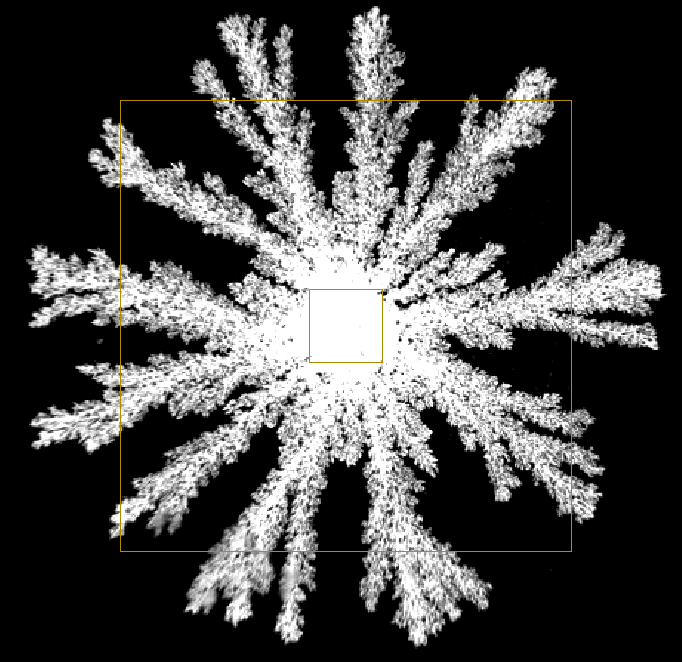
\includegraphics[width=0.5\textwidth]{radius_cutting_img.png} & 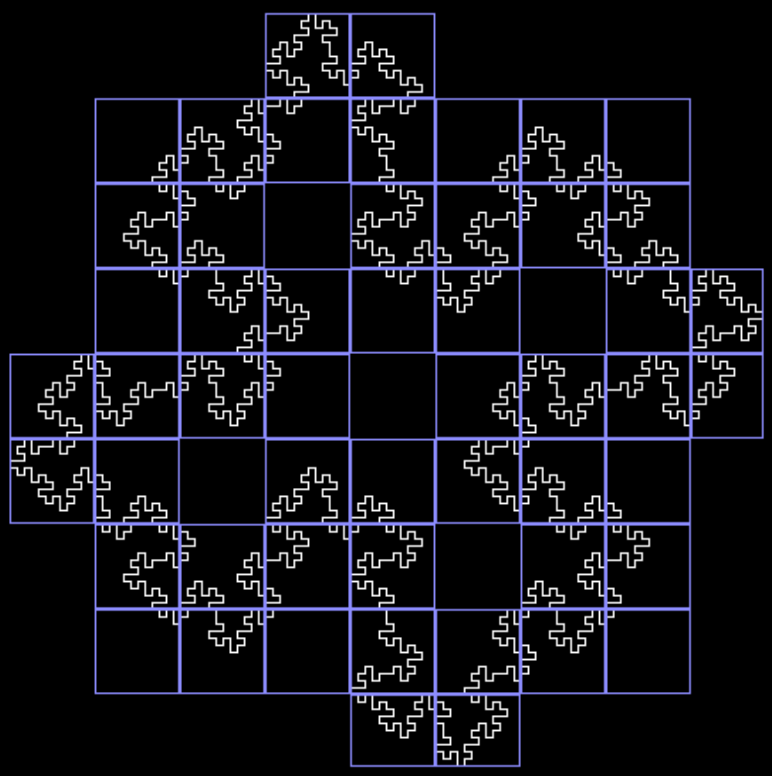
\includegraphics[width=0.5\textwidth]{Boxcounting.png}\\
                (a) & (b)
        \end{tabular}
        \caption{\label{fig:radiuscutting}Illustration of the dimension estimation methods. (a) Shows the effect of varying included $r$ values, as indicated by the thin yellow lines, in the mass-radius method. Note that they are chosen such that the area of the filled centre and outer empty area inside the considered zone are minimised. (b)(\cite{ImageJ}) Shows an example of the box counting method, where the fractal is covered by a mesh of boxes of size $s$.}
\end{figure}

\indent In our analysis we categorise our fractals as in \cite{PhysRevLett.56.1260}, in four categories:
\begin{enumerate}
        \item \textbf{Stringy} - Fractals which are made up of long thin branches.
        \item \textbf{Open} - Thick open ramified structures that, while fractal, dont show particularly fine structure.
        \item \textbf{Dendritic} - Many large branches, with similar smaller branches offshooting, significant fractal behaviour and self similarity. 
        \item \textbf{Homogeneous} - In these fractals, the zinc deposits spread uniformly over the cathode, and the fractal dimension closer to 2.
\end{enumerate}






\section{Methodology}\label{sec:methodology}
The procedure of this experiment begins with the preparation of the zinc sulphate monohydrate solution. We first find the molar mass of zinc sulphate monohydrate, which has the formula $ZnSO_4H_2O$.
\begin{align*}
        M_{ZnSO_4H_2O} &= M_{Zn} + M_{S} + 4M_{O} + 2M_{H} + M_{O} = 65\\
        M_{ZnSO_4H_2O} &= 65.38 + 32.066 + 4(16.000) + 2(1.008) + 16.000 = 179.462\text{ g/mol}
\end{align*}
We then make samples of concentrations 1M, 0.25M, 0.1M and 0.01M, by first making $200$ml of 1M solution ($200ml$ deionised water, $39.892g$ of $ZnSO_4H_2O$), and then diluting appropriately with deionised water.
\indent While making the 1M solution balance was used to measure the volume of water and mass of $ZnSO_4H_2O$. The $ZnSO_4H_2O$ was ground in a pestle and mortar to remove clumps from the powder, and then added slowly to the water, stirring continuously to ensure a homogeneous solution without undisolved $ZnSO_4H_2O$ remaining. When diluting further some of this solution, measurements were taken using a $50ml$ lab syringe, and mixing in a beaker with an aappropriate amount of deionised water.\\
\indent The configuration of the experiment was similar to that in (\cite{PhysRevLett.56.1260}), where the solution is placed in a very shallow cylindrical gap between a plexiglass plate, and a disk fitting into the gap, with a conducting ring on the edge, and a graphite stick entering through a hole in the centre of the upper disk. Both the ring and the stick are connected to a power supply, with the graphite acting as the cathode and ring as the anode. The voltage across the solution is kept constant, and the zinc from the $ZnSO_4H_2O$ deposits on the cathode, becoming a part of it. The fractal growth due to this continual deposition is then observed and recorded.\\
\indent The fractal growth is recorded using a camera, and while usually in this experiment the lab software ImageJ, and Benoit would be used to manipulate the images, and analyse the fractals respectively, in this case, due to time constraints, these tasks were done using GIMP and Fractalyse, a fractal analysis software written in java which can be found \href{https://sourcesup.renater.fr/www/fractalyse/}{here}. I would recommend the use of this software, as it is very user friendly, and has a lot of features which are useful for the analysis of fractals.\\
\indent Both the box counting and the mass-radius methods (outlined in \ref{sec:background}) of fractal analysis were used in this experiment to find the fractal dimensions of the samples.
\section{Results}



\section{Discussion}



\addcontentsline{toc}{section}{\numberline{}Appendix}
\section*{Appendix}



\bibliographystyle{plainnat}
\bibliography{references}

\end{document}